\documentclass[ignorenonframetext,]{beamer}
% EJ latex definitions and style
\newcommand*\diff{\mathop{}\!\mathrm{d}}
\newcommand*\red{\color{red}}
\setbeamertemplate{caption}[numbered]
\setbeamertemplate{caption label separator}{:}
\setbeamercolor{caption name}{fg=normal text.fg}
\usepackage{amssymb,amsmath}
\usepackage{ifxetex,ifluatex}
\usepackage{fixltx2e} % provides \textsubscript
\usepackage{lmodern}
\ifxetex
  \usepackage{fontspec,xltxtra,xunicode}
  \defaultfontfeatures{Mapping=tex-text,Scale=MatchLowercase}
  \newcommand{\euro}{€}
\else
  \ifluatex
    \usepackage{fontspec}
    \defaultfontfeatures{Mapping=tex-text,Scale=MatchLowercase}
    \newcommand{\euro}{€}
  \else
    \usepackage[T1]{fontenc}
    \usepackage[utf8]{inputenc}
      \fi
\fi
% use upquote if available, for straight quotes in verbatim environments
\IfFileExists{upquote.sty}{\usepackage{upquote}}{}
% use microtype if available
\IfFileExists{microtype.sty}{\usepackage{microtype}}{}
\usepackage{graphicx}
\makeatletter
\def\maxwidth{\ifdim\Gin@nat@width>\linewidth\linewidth\else\Gin@nat@width\fi}
\def\maxheight{\ifdim\Gin@nat@height>\textheight0.8\textheight\else\Gin@nat@height\fi}
\makeatother
% Scale images if necessary, so that they will not overflow the page
% margins by default, and it is still possible to overwrite the defaults
% using explicit options in \includegraphics[width, height, ...]{}
\setkeys{Gin}{width=\maxwidth,height=\maxheight,keepaspectratio}

% Comment these out if you don't want a slide with just the
% part/section/subsection/subsubsection title:
\AtBeginPart{
  \let\insertpartnumber\relax
  \let\partname\relax
  \frame{\partpage}
}
\AtBeginSection{
  \let\insertsectionnumber\relax
  \let\sectionname\relax
  \frame{\sectionpage}
}
\AtBeginSubsection{
  \let\insertsubsectionnumber\relax
  \let\subsectionname\relax
  \frame{\subsectionpage}
}

\setlength{\parindent}{0pt}
\setlength{\parskip}{6pt plus 2pt minus 1pt}
\setlength{\emergencystretch}{3em}  % prevent overfull lines
\setcounter{secnumdepth}{0}
\usepackage[]{algorithm2e}

\title{\(0^{\text {th}}\) order model for competing microbes}
\author{Eric Jones}
\date{}

\begin{document}
\frame{\titlepage}

\begin{frame}{Background}

\begin{itemize}
\itemsep1pt\parskip0pt\parsep0pt
\item
  Derived from the plankton-rotifer trait-based predator-prey model
  (\texttt{http://dx.doi.org/10.1016/j.ecolmodel.2009.05.005}) by
  Agostino Merico
\item
  \(n\) and \(m\) types of microbes A and B; each of the A-type microbes
  share the same death rate \(\mu_A\), but has a stochastic growth rate
  which provides variety within a given microbe
\item
  In addition, of the \(1 - \kappa\) energy available for the microbe, a
  proportion \(\delta_{A_i}\) goes to defense and \(\alpha_{A_i}\) goes
  to nutrient allocation
\item
  This model assumes that the microbes compete for nutrients, but
  otherwise do not interact with each other (hence a 0\(^\text{th}\)
  order model)
\item
  When microbes die, we assume their biomass is returned into the
  existing nutrients, \(N\)
\item
  Next steps: fit the model to data (\textbf{\emph{which constants?}}),
  add in intermicrobe interaction, add in immune system interaction
\end{itemize}

\end{frame}

\begin{frame}{Model}

\begin{align*}
    \frac{\diff A_1}{\diff t} &= \left[ {\red \gamma_A} \left(
    \frac{N}{N + \frac{\color{red} K_{A}}{\alpha_{A_1}}}\right) - {\red \mu_A}
    \right]A_1\\ \vdots & \\
    \frac{\diff A_n}{\diff t} &= \left[ {\red \gamma_A} \left( \frac{N}{N +
    \frac{\color{red} K_{A}}{\alpha_{A_n}}}\right) - {\red \mu_A} \right]A_n\\
    \frac{\diff B_1}{\diff t} &= \left[ {\red \gamma_B} \left(
    \frac{N}{N + \frac{\color{red} K_{B}}{\alpha_{B_i}}}\right) - {\red \mu_B}
    \right]B_1\\ \vdots & \\
    \frac{\diff B_m}{\diff t} &= \left[ {\red \gamma_B} \left(
    \frac{N}{N + \frac{\color{red} K_{B}}{\alpha_{B_m}}}\right) - {\red \mu_B}
    \right]B_m\\ \frac{\diff N}{\diff t} &= - \sum_i \left( \frac{\diff
    A_i}{\diff t} + \frac{\diff B_i}{\diff t}  \right) + \beta(N_0 - N)
\end{align*}

\end{frame}

\begin{frame}{Fitting Data}

\begin{itemize}
\itemsep1pt\parskip0pt\parsep0pt
\item
  Initially, we try to fit parameters for just one species of microbe

  \begin{align*}
  \frac{\diff A}{\diff t} &= \left[ {\red \gamma} \left( \frac{N}{N +
  {\color{red} K}}\right) - {\red \mu} \right]A \\
  \frac{\diff N}{\diff t} &= - \frac{\diff A}{\diff t} + 
  \beta(N_0 - N)
  \end{align*}
\item
  From the experimental design, we should know \(\beta\) and \(N_0\)
\item
  We need to fit \({\red \gamma, \ K}\), and \({\red \mu}\) from data
\end{itemize}

\end{frame}

\begin{frame}{``Experimental'' Data}

\begin{figure}[htbp]
\centering
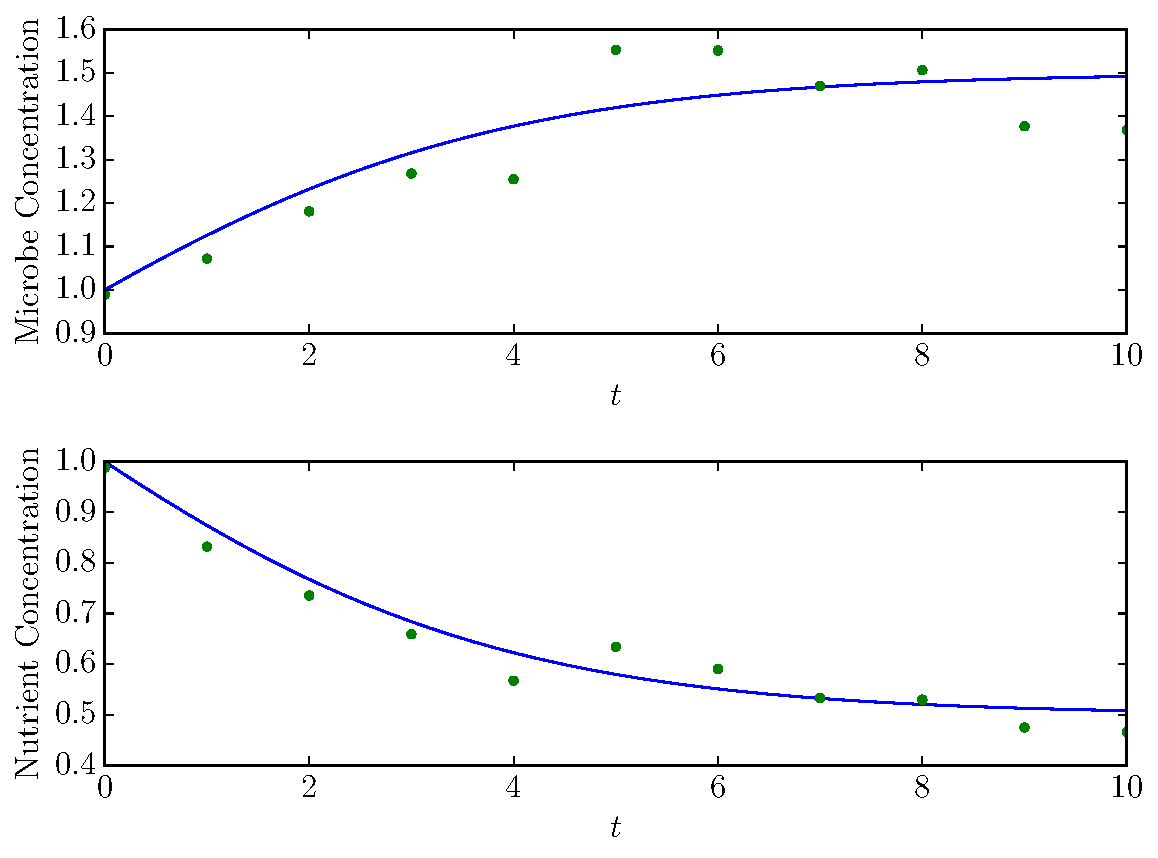
\includegraphics{one_microbe.pdf}
\caption{Data from model with random fluctuations}
\end{figure}

\end{frame}

\begin{frame}{Univariate Bayesian Parameter Estimation}

\KwData{$\hat{y}$ dependent on $\theta_\text{true}$ at $n$ time-steps, with
model $y(\theta_\text{guess})$ at any time-steps} set range for possible
\(\theta\) values
(\([\theta] = [\theta_\text{min}, \ldots, \theta_\text{max}]\));\\\For{each $\theta[i]$}{
    \textit{set initial uniform prior:}\; \\
    probability[i,0] = 1\; \\
    \For{each timestep $j$}{
        $y_{i,j} = y(\theta[i])|_{t=j}$\; \\
        \textit{compare data to proposed $\theta$ value}:\; \\
        distance$[i,j]$ = \texttt{normalpdf}($\hat{y}(t=j), \mu=y_{i,j},
        \sigma^2 = 1 )$\; \\
        probability$[i,j]$ = probability$[i,j-1]$*distance$[i,j]$
    }
} normalize probabilities;

\textbf{As the number of time steps increases, the probability
distributions over \(\theta\) should approach \(\theta_\text{true}\)}

\end{frame}

\end{document}
